\documentclass[letter,11pt]{article}

\usepackage[margin=1in]{geometry}
\usepackage[utf8]{inputenc}
\usepackage{color}
\usepackage{xcolor}
\usepackage{amsmath}
\usepackage{amssymb}
\usepackage{amsthm}
\usepackage{hyperref}
\usepackage{graphicx}
\usepackage{tikz}
\usepackage{caption}
\usepackage{float}
\usepackage[shortlabels]{enumitem}
\usetikzlibrary{positioning,arrows.meta}

\usepackage[plain]{algorithm}
\usepackage{algorithmicx}
\usepackage[]{algpseudocode}




\begin{document}

\noindent\rule[2mm]{\textwidth}{1.5mm}
\noindent
\begin{minipage}{.3\textwidth}
  \vspace{-3mm}
  {\Huge\bf HW 5}
\end{minipage}\hfill\begin{minipage}{.5\textwidth}
\begin{flushright}
  {\bf Intro Algorithms EN.601.433 \\
  Fall 2023 \\
  Due: Friday 11/10/2023 at 11:59 PM}%
\vspace{3mm}
\end{flushright}
\end{minipage}
\noindent\rule{\textwidth}{1.5mm}

\section*{Instructions}

\begin{itemize}
\item This homework is worth 10\% of your final grade.

\item This homework is due Friday 11/10/2023 at 11:59 PM on Gradescope.  Solutions will be posted on Canvas at midnight.  No late homework will be accepted.  To access Gradescope, click the Gradescope link on Canvas.

\item You are \textbf{required} to type your homework.  We will
  provide the \LaTeX{} source code to the homework assignments, which you may
  optionally use as a template.  If you install \LaTeX{} on your computer, you can
  generate a PDF of
  your homework by running the command: \\
  \\
  \texttt{latexmk~-pdf~my-homework.tex} \\
  \\
  Alternately, you can use \url{https://www.overleaf.com/edu/jhu} as a web based
  \LaTeX{} editor.

\item You can collaborate with one other person.
    Collaboration should happen through verbal communication, scratch paper,
    whiteboards, etc.  You are \textbf{not} allowed to copy homework
    solutions from another student.  All students are required to submit their
    own write-up.

\item You are \textbf{not} allowed to use any website to find solutions to these problems.

\item Do not write your name on your homework. Instead, write your Johns Hopkins Student ID.  This will allow us to grade your homework anonymously.

\item For questions that require you to write an algorithm out, you can either use pseudo-code or English description.

\item Make sure that you correctly assign which page a problem is located on when uploading to Gradescope.

\item For problems that require graphs or diagrams, you are allowed to include an image of a drawing instead of typesetting the graph.\footnote{If you are using LaTeX, you can follow the instructions here \url{https://www.overleaf.com/learn/latex/Inserting_Images} to embed an image in LaTeX.}

\item \textbf{For each problem in this homework: define the optimizing function, define the Bellman equation, give the algorithm to compute the optimizing function and give a brief justification for the runtime.}
\end{itemize}


\newpage
%%%%%%%%%%%%%%%%%%%%%%%%%%%%%%%%%%%%%%%%%%%%%%%%%%%%%%%%%%%%%%%%%%%%%%%%%%%%%%%%%%%%%%%%%%%%%%%%%%%%
%  _    ___          __  _____           _     _
% | |  | \ \        / / |  __ \         | |   | |
% | |__| |\ \  /\  / /  | |__) | __ ___ | |__ | | ___ _ __ ___  ___
% |  __  | \ \/  \/ /   |  ___/ '__/ _ \| '_ \| |/ _ \ '_ ` _ \/ __|
% | |  | |  \  /\  /    | |   | | | (_) | |_) | |  __/ | | | | \__ \
% |_|  |_|   \/  \/     |_|   |_|  \___/|_.__/|_|\___|_| |_| |_|___/
%%%%%%%%%%%%%%%%%%%%%%%%%%%%%%%%%%%%%%%%%%%%%%%%%%%%%%%%%%%%%%%%%%%%%%%%%%%%%%%%%%%%%%%%%%%%%%%%%%%%

\section{Longest Path in a Graph (6 points)}

Let $G=(V,E)$ be a directed graph with nodes $v_1,\dots,v_n$. We say that $G$ is an ordered graph if it has the following properties.

\begin{enumerate}
    \item [i] Each edge goes from a node with a lower index to a node with a higher index. That is, every directed edge has the form $(v_i,v_j)$ with $i<j$.
    \item [ii] Each node except $v_n$ has at least one edge leaving it. That is, for every node $v_i,$ where $i=1,2,\dots,n-1$, there is at least one edge of the form $(v_i,v_j)$.
\end{enumerate}

\textbf{Goal:} \textit{Given an ordered graph $G$, find the length of the longest path that begins at $v_1$ and ends at $v_n$.} The length of a path is the number of edges in it.

\begin{figure}[H]
  \centering
  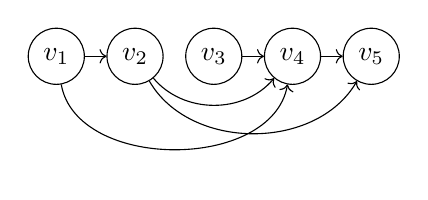
\begin{tikzpicture}
    \node[circle,draw] (v1) {$v_1$} ;
    \node[circle,draw,right of=v1] (v2) {$v_2$} ;
    \node[circle,draw,right of=v2] (v3) {$v_3$} ;
    \node[circle,draw,right of=v3] (v4) {$v_4$} ;
    \node[circle,draw,right of=v4] (v5) {$v_5$} ;
    \draw[->] (v1) -- (v2) ;
    \draw[->] (v3) -- (v4) ;
    \draw[->] (v4) -- (v5) ;
    \draw[->] (v1) to[bend right=80] (v4) ;
    \draw[->] (v2) to[bend right=50] (v4) ;
    \draw[->] (v2) to[bend right=60] (v5) ;
  \end{tikzpicture}
  \caption{The longest path from $v_1$ to $v_n$ uses 3 edges $(v_1,v_2)$, $(v_2, v_4)$, $(v_4, v_5)$.}
\end{figure}

\begin{enumerate}
  
\item Show that the following algorithm does not correctly solve this problem, by giving an example of an ordered graph on which it does not return the correct answer

\begin{algorithm}[H]
    \caption{``Longest Path'' Greedy Algorithm}
    \begin{algorithmic}
        \State Set $w=v_1$
        \State Set $L=0$
        \While{there is an edge out of the node $w$}
        \State Chose the edge $(w, v_j)$ for which $j$ is as small as possible
        \State Set $w=v_j$
        \State Increment $L$ by $1$
        \EndWhile \\
        \Return $L$ as the length of the longest path
    \end{algorithmic}
\end{algorithm}

\item Give an efficient algorithm that takes an ordered graph $G$ and returns the length of the longest path that begins at $v_1$ and ends at $v_n$. (Again, the length of a path is the number of edges in the path.)
\end{enumerate}

\subsection{Solution: Ordered Graph Counterexample}

\[\includegraphics[width=10cm]{q1 graph.png}\]
\[\text{Counterexample: Gives length 2 as the longest path from V1 to V5, but should be 3.}\]

\subsection{Solution: Efficient Algorithm}

Let $G=(V,E)$ be an ordered, directed graph with nodes $v_1,\dots,v_n$. For $i = 1, \dots, n$, let $L[i]$ be the length of the longest path from $v_1$ to $v_n$. In this case, $L[1] = 0$, because the only path from $v_1$ to $v_1$ is the one with no path, since there are no cycles. For $i = 2, \dots, n$:

\[L[i] = \text{max}\{1 + L[j] : (v_j,v_i) \in E \}\]

This means that a longest path from $v_1$ to $v_i$ is made up from a longest path $v_1$ to $v_j$ followed by the edge $(v_j, v_i)$, for some $j < i$. We set $L[i] = -\infty$ if there does not exist an edge $(v_j, v_i)$.

To calculate the longest paths, we use another array $P$ to store the predecessor of $i$ on the longest path from $v_1$ to $v_i$ while computing the values of L.\\

\noindent $L[1] = 0$;\\
$P[1] = 0$;\\
for $i = 2, \dots, n$: \\
\indent $L[i] = -\infty$;\\
\indent $P[i] = -1$;\\
\indent for $(v_j, v_i) \in E$:\\
\indent \indent if $1 + L[j] > L[i]$:\\
\indent \indent \indent $L[i] = 1 + L[j]$;\\
\indent \indent \indent $P[i] = j$\\
return $L[n]$;









\section{Formatting Text (4 points)}

In a word processor, the goal of ``pretty-printing'' is to take text with a ragged right margin, like this,

\begin{verbatim}
Call me Ishmael.
Some years ago,
never mind how long precisely,
having little or no money in my purse,
and nothing particular to interest me on shore,
I thought I would sail about a little
and see the watery part of the world.
\end{verbatim}

and turn it into text whose right margin is as ``even'' as possible, like this,

% \begin{figure}[H]
%     \begin{subfigure}[H]{0.7\linewidth}
%     \centering
%     \includegraphics[width=1\linewidth]{q3.png}
%     \end{subfigure}
%     \setlength{\belowcaptionskip}{-10pt}
%     \label{fig:q3}
% \end{figure}

\begin{verbatim}
Call me Ishmael. Some years ago, never
mind how long precisely, having little
or no money in my purse, and nothing
particular to interest me on shore, I
thought I would sail about a little
and see the watery part of the world.
\end{verbatim}

To make this precise enough for us to start thinking about how to write a pretty-printer for text, we need to figure out what it means for the right margins to be ``even.'' So suppose our text consists of a sequence of words, $W={w_1,w_2,\dots,w_n}$, where $w_i$ consists of $c_i$ characters. We have a maximum line length of $L$. We will assume we have a fixed-width font and ignore issues of punctuation or hyphenation.

A formatting of $W$ consists of a partition of the words in $W$ into lines. In the words assigned to a single line, there should be a space after each word except the last; and so if $w_j,w_{j+1},\dots,w_k$ are assigned to one line, then we should have

\begin{center}
    $[\sum_{i=j}^{k-1} (c_i + 1)] + c_k \leq L$
\end{center}

We will call an assignment of words to a line valid if it satisfies this inequality. The difference between the left-hand side and the right-hand side will be called the slack of the line—that is, the number of spaces left at the right margin.

Give an efficient algorithm to find a partition of a set of words $W$ into valid lines, so that the sum of the squares of the slacks of all lines (including the last line) is minimized.

\subsection{Solution: Algorithm}

Our optimizing function solution of $i$ is the minimum cost of the set of words $w_1, \dots, w_i$. Let $S_{i,j}$ be the slack of the line consisting of words $w_i,\dots,w_j$. The algorithm equation is as follows:

\[ \text{OPTIMAL}[i] = \min \{ S^2_{i,n} + \text{OPTIMAL}[j - 1] \}, 1 \leq j \leq n\]

\noindent The algorithm is as follows: \\
For $j = 1$ to $n$:\\
\indent For $i = 1$ to $j$:\\
\indent \indent Compute all $S_{i,j}$ values for $w_i,\dots,w_j$;\\
Initialize array $M$ and set $M[0] = 0$;\\
For $j = 1$ to $n$:\\
\indent $M[j] = \min_{1 \leq i \leq j} \{ S^2_{i,j} + \text{OPTIMAL}[i - 1] \}$\\
Return $M[n]$\\






\section{This is Zion and we are not afraid! (6 points)}
The residents of the underground city of Zion defend themselves through a combination of kung fu, heavy artillery, and efficient algorithms. Recently they have become interested in automated methods that can help fend off attacks by swarms of robots.\footnote{This problem is a reference to The Matrix Trilogy \url{https://en.wikipedia.org/wiki/The_Matrix_(franchise)}, specifically the third movie in the series: The Matrix Revolutions.}

Here’s what one of these robot attacks looks like.

\begin{itemize}
    \item A swarm of robots arrives over the course of $n$ seconds; in the $i$-th
    second, $x_i$ robots arrive. Based on remote sensing data, you know this sequence $x_1, x_2 , ..., x_n$ in advance.

    \item You have at your disposal an \textit{electromagnetic pulse} (EMP), which can destroy some of the robots as they arrive; the EMP's power depends on how long it's been allowed to charge up. To make this precise, there is a function $f(\cdot)$ so that if $j$ seconds have passed since the EMP was last used, then it is capable of destroying up to $f(j)$ robots.

    \item So specifically, if it is used in the $k$-th second, and it has been $j$ seconds since it was previously used, then it will destroy $min(x_k , f(j))$ robots. After this use, it will be completely drained.

    \item We will also assume that the EMP starts off completely drained, so if it is used for the first time in the $j$-th second, then it is capable of destroying up to $f(j)$ robots.
\end{itemize}

{\bf The Problem.} Given the data on robot arrivals $x_1, x_2 , ..., x_n$ , and given the recharging function $f(\cdot)$, choose the points in time at which you're going to activate the EMP so as to destroy as many robots as possible.

\textbf{Example}: Suppose $n=4$ and the values of $x_i$ and $f(i)$ are given by the table below.

\begin{center}
\begin{tabular}{|c|c|c|c|c|}
    \hline
    i & 1 & 2 & 3 & 4 \\
    \hline
    $x_i$ & 1 & 10 & 10 & 1 \\
    $f(i)$ & 1 & 2 & 4 & 8 \\
    \hline
\end{tabular}
\end{center}

The best solution would be to activate the EMP in the $3^{rd}$ and the $4^{th}$ seconds. In the $3^{rd}$ second, the EMP has gotten to charge for 3 seconds, and so it destroys $min(10, 4) = 4$ robots. In the $4^{th}$ second, the EMP has only gotten to charge for 1 second since its last use, and it destroys $min(1, 1) = 1$
robot. This is a total of 5.

\begin{enumerate}
    \item[a)] Show that {\bf Algorithm \ref{algo:emp_schedule_bad}} does not correctly solve this problem,
    by giving an instance on which it does not return the correct answer.
    In your example, say what the correct answer is and also the output of {\bf Algorithm \ref{algo:emp_schedule_bad}}.

    \begin{algorithm}
        \caption{EMP-scheduling algorithm}
        \begin{algorithmic}
            \Function{Schedule-EMP}{$x_1, ..., x_n$}
                \State Let $j$ be the smallest number such that $f(j) \geq x_n$ \\
                \Comment{(If no such $j$ exists, set $j = n$)}
                \State Activate EMP in $n^{th}$ second
                \If{$n-j \geq 1$}
                    \State Schedule-EMP($x_1, ..., x_{n-j}$)
                \EndIf
            \EndFunction
          \end{algorithmic}
          \label{algo:emp_schedule_bad}
    \end{algorithm}


  \item[b)] Give an efficient algorithm that takes the data on robot arrivals $x_1, x_2, ..., x_n$ and the recharging function $f(\cdot)$ and returns the maximum number of robots that can be destroyed by a sequence of EMP activations.

%    Write out your algorithm in the form of a Bellman equation and a function which computes the result.

    
%    \item[c)] What is the running time of your proposed algorithm? Briefly justify the run time calculations.
\end{enumerate}

\subsection{Solution: Counterexample}

Let n = 5, f(1) = 1, f(2) = 2, f(3) = 3, f(4) = 4, f(5) = 5; and x1 = 2, x2 = 3, x3 = 4, x4 = 1,
x5 = 5. Then the algorithm above will activate EMP in second 4, while activating in seconds 3 and 5 is better

\subsection{Solution: Algorithm}

Let OPTIMAL$(j)$ be the maximum number of robots that can be destroyed for the problem from $x_1,\dots,x_j$. Since the input ends at $x_j$, we don't need to activate it then, because we aren't saving it for anything. Therefore, we must choose when to activate it before $j$. Therefore:

\[\text{OPTIMAL}(j) = \max [\text{OPTIMAL}(i) + \min \{ x_j, f(j-i) \}], 0 \leq i < j\]

\noindent The algorithm is as follows:

\noindent Set OPTIMAL$(0) = 0$;\\
For $j = 1 \rightarrow n$;\\
\indent compute OPTIMAL$(j)$ using above formula;\\
return OPTIMAL$(n)$;\\





\section{Smart Stock Surge (4 points)}
Imagine you're looking at the price of a given stock over $n$ consecutive days, numbered $i = 1, 2, \ldots, n$. For each day $i$, we have a price $p(i)$ per share for the stock on that day. We'll assume for simplicity that the price was fixed during each day. How should we choose a day $i$ on which to buy the stock and a later day $j > i$ on which to sell it, if we want to maximize the profit per share, $p(j) - p(i)$? If there is no way to make money during the $n$ days, we should conclude this instead. Show how to find the optimal pair of days $i$ and $j$ in time $O(n)$ using Dynamic Programming. 

\subsection{Solution: Algorithm Explanation}

Our optimal function OPTIMAL$(i)$ is the maximum profit made from buying a stock on day $i$ and selling it on a later day $j > i$. Our algorithm equation is as follows:

\[\text{OPTIMAL}(i) = \max \{ p(j) - p(i) : j > i \}\]

If there is no way to make money, the maximum profit is 0, so OPTIMAL$(n)$ = 0. Our algorithm is as follows:

\noindent Initialize maximum profit as $0$;\\
Initialize the minimum price as $p(1)$;\\
If $n \leq 1$, Return $0$;\\
For $i = 2$ to $n$:\\
\indent If $p(i) <$ minimum price:\\
\indent \indent minimum price $= p(i)$;\\
\indent current profit $= p(i) -$ minimum price;\\
\indent If current profit $>$ maximum profit:\\
\indent \indent maximum profit $=$ current profit;\\
Return the maximum profit.\\


\section{Longest Rising Trend in Stock Prices (6 points)}
Your friends have been studying the closing prices of tech stocks, looking for interesting patterns. They've defined something called a \textit{rising trend}, as follows:
They have the closing price for a given stock recorded for $n$ days in succession; let these prices be denoted $P[1], P[2], \ldots , P[n]$. A \textit{rising trend} in these prices is a subsequence of the prices $P[i], P[j], \ldots, P[k]$ for days $i < j < \ldots < k$ so that
\begin{itemize}
    \item $i = 1$, and
    \item $P[j] < P[j+1]$ for each $j = 1,2, \ldots, k-1$.
\end{itemize}
Thus a rising trend is a subsequence of the days - beginning on the first day and not necessarily contiguous - so that the price strictly increases over the days in this subsequence.

They are interested in finding the longest rising trend in a given sequence of prices.

\textbf{Example:} Suppose $n=7$, and the sequence of prices is
\[10, 1, 2, 11, 3, 4, 12\]

Then the longest rising trend is given by the prices on days 1, 4, and 7. Note that days 2, 3, 5, and 6 consist of increasing prices; but because this subsequence does not begin on day 1, it does not fit the definition of a rising trend.

\subsection*{(a)}
Show that the following algorithm does not correctly return the length of the longest rising trend, by giving an instance on which it fails to return the correct answer.
\begin{verbatim}
Define i = 1
L = 1
For j = 2 to n
    If P[j] > P[i] then
        Set i = j
        Add 1 to L
    Endif
Endfor
\end{verbatim}
In your example, give the actual length of the longest rising trend, and say what the algorithm above returns.

\subsection*{(b)}
Give an efficient algorithm that takes a sequence of prices $P[1], P[2], \ldots, P[n]$ and returns the {\it length} of the longest rising trend.

\subsection{Solution: Counterexample}

Suppose $n = 8$, and the sequence of prices issues
\[1, 7, 2, 3, 4, 10, 6, 12\]

Then, the given algorithm will give us that the longest rising trend is length 3, calculating the subsequence
\[1, 7, 10, 12\]
when in fact, the actual longest rising trend should be length 5, with subsequence 
\[1, 2, 3, 4, 6, 12\].

\subsection{Algorithm}

For our algorithm, our optimal solution is the length of the longest rising trend ending at index $i$, starting at the first day. Therefore, our equation is as follows:

\[\text{OPTIMAL}(i) = \max \{ \text{OPTIMAL}(i), \text{OPTIMAL}(j) + 1 \}\]

\noindent The algorithm is as follows: \\
Initialize an array $L$ and set $L[0] = 1$, since the length of the longest rising trend at the first index is always $1$.\\
For $i = 1$ to $n - 1$:\\
\indent For $j = 0$ to $i - 1$:\\
\indent \indent If $P[i] > P[j]$:\\
\indent \indent \indent $L[i] = \max\{ L[i], L[j + 1]\}$\\
Maximum length $=$ maximum value in array $L$\\
Return the maximum length;\\


\section{You shall not fail! (7 points)}
Suppose it’s nearing the end of the semester and you’re taking $n$ courses, each with a final project that still has to be done. Each project will be graded on the following scale: It will be assigned an integer number on a scale of 1 to $g > 1$, higher numbers being better grades. Your goal, of course, is to maximize your average grade on the $n$ projects.

You have a total of $H > n$ hours in which to work on the $n$ projects cumulatively, and you want to decide how to divide up this time. For simplicity, assume $H$ is a positive integer, and you’ll spend an integer number of hours on each project. To figure out how best to divide up your time, you’ve come up with a set of functions \{$f_i :i = 1, 2,\ldots,n$\} (rough estimates, of course) for each of your n courses; if you spend h $\leq$ H hours on the project for course $i$, you’ll get a grade of $f_i(h)$. (You may assume that the functions $f_i$ are nondecreasing: if $h < h'$, then $f_i(h) \leq f_i(h')$.)

So the problem is: Given these functions $\{f_i\}$, decide how many hours to spend on each project (in integer values only) so that your average grade, as computed according to the $f_i$, is as large as possible. In order to be efficient, the running time of your algorithm should be polynomial in $n$, $g$, and $H$; none of these quantities should appear as an exponent in your running time.\\



\textbf{Use your algorithm to solve the following example}:
You are taking 3 courses C++, Java and Python $(n=3)$ and you have a total of 5 hours $(H=5)$ to work on the projects. The functions $f_i$ for each course is as follows:

\begin{center}
\begin{tabular}{|l|c|c|c|c|c|c|}
\hline
Hours spent & 0 & 1 & 2 & 3 & 4 & 5 \\
\hline
C++ grades & 0 & 1 & 3 & 5 & 5 & 5 \\ 
\hline
Java grades & 0 & 3 & 3 & 4 & 5 & 6 \\ 
\hline
Python grades & 0 & 1 & 4 & 4 & 4 & 7 \\ 
\hline
\end{tabular}
\end{center}
Use your algorithm to find the optimal distribution of time to maximize the total grade. Your algorithm should output the maximum grades achieved. Calculate the number of hours spent on each course.

\subsection{Solution: Algorithm}

We need to maximize the total grade over $n$ courses while spending $H$ hours. We can split this problem into multiple $(i, h)$ subproblems, where an $(i,h)$-subproblem is the problem where we want to maximize the total grade over the first $i$ courses by using at most $h$ hours.

Let $A[i,h]$ be the maximum total grade that can be achieved with the $(i,h)$ subproblem. In this case, $A[0,h] = 0$ for all $h$, and $A[i,0] = \sum_{j = 1}^{i} f_j(0)$. In the optimal solution, we spend $k$ hours on course $i$ for some value of $k \in [0,h]$. Therefore, our algorithm equation is as follows:

\[A[i,h] = \max \{f_i(k) + A[i-1,h-k]\}, 0 \leq k < h\]

From the output $A[n, H]$, we can trace back the entries using the recorded values to produce the optimal result. So to find a specific amount of hours $k$ to spend on a class, we backtrack through the solution to find the solution. The total time to fill each entry $A[i,h]$ is $O(h)$, and since there are $n * H$ entries, the total runtime is $\mathcal{O}(nH^2)$.

\subsection{Solution: Solving the Example}

The maximum total grade received is 10, spending 2 hours on C++, 1 hour on Java, and 2 hours on Python.



\end{document}
